% Provenance (never printed): lycee terminale S SVT "Les climats de la Terre"
% and the 2019 enseignement scientifique ("Le climat de la Terre": forcing,
% feedbacks, the IPCC assessments, scenarios), union; physical science only,
% as the user ruled (2026-10-22). See sources/outline_sources.md. Pilot
% chapter, 2026-10-22. Every figure about the climate system is an IPCC AR6
% WG1 statement (ledger ipcc:*) or computed from a dataset in
% figdata/grade-12/climate_records.py.
\chapter{Klimaatverandering: waarnemingen, oorzaken en projecties}\label{ch:g12:climate-change}

Hoog op de noordhelling van Mauna Loa, een vulkaan midden in de
Grote Oceaan, staat een groepje witte gebouwen op kale lava,
\qty{3397}{m} boven de zee. Daarboven, boven de luchtlaag die vervuild wordt door
het eiland eronder en duizenden kilometers van elke grote stad, is de lucht
ongeveer even zuiver en goed gemengd als de atmosfeer van de hele planeet. Sinds
maart 1958 wordt het koolstofdioxide er bijna zonder onderbreking gemeten.
De reeks begon als het project van één scheikundige; ze is de beroemdste
kromme van de aardwetenschappen geworden. Dit hoofdstuk leest die kromme en de andere reeksen
van het klimaat, legt uit hoe een verandering in de lucht het energiebudget
van de planeet verandert, hoe wetenschappers beslissen wat de opwarming veroorzaakte die ze waarnemen,
en wat ze voor de komende decennia projecteren.
% ledger: noaa:mlo-site, noaa:keeling-1958

\begin{omfigure}
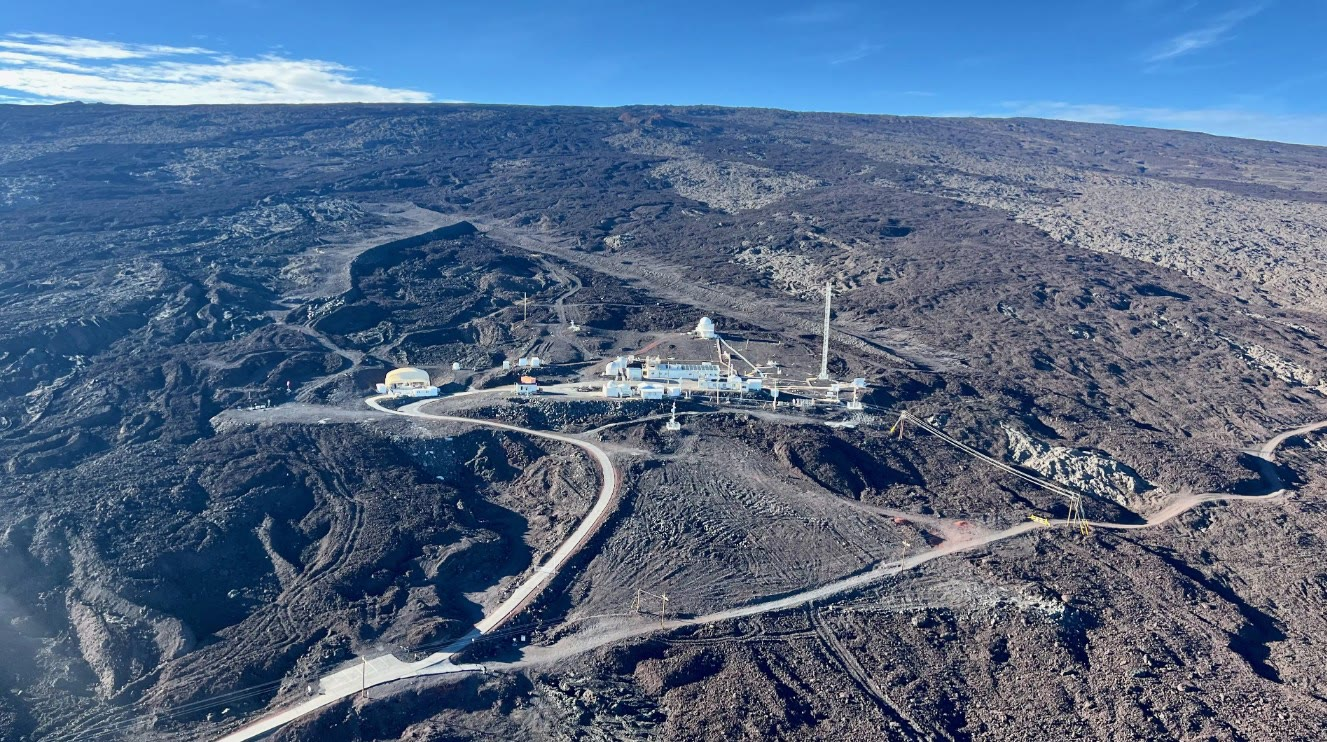
\includegraphics[width=0.78\linewidth]{images/book2/g12-noaa-mauna-loa-observatory.jpg}

{\small Het Mauna Loa Observatory, Hawaï, op oude lavastromen hoog op de
noordflank van de vulkaan. Foto: Brian Vasel, NOAA (publiek domein).}
\end{omfigure}

\begin{recall}
De Aarde ontvangt energie van de Zon als licht en verliest gemiddeld evenveel
aan de ruimte als infraroodstraling; de fractie zonlicht die wordt teruggekaatst,
is het \omterm{def:g10:earth-energy-budget:albedo}{albedo} (\cref{ch:g10:earth-energy-budget}). Broeikasgassen --- waterdamp,
koolstofdioxide, methaan --- absorberen een deel van het infrarood dat het
oppervlak uitzendt en sturen een deel ervan terug naar beneden; dit broeikaseffect houdt
het oppervlak veel warmer dan het anders zou zijn (de scheikundeboeken, en
Boek 1, jaar 9). IJskernen bewaren belletjes oude lucht en leggen de
glaciale cycli van de laatste 800\,000 jaar vast (\cref{ch:g12:past-climates}).
\end{recall}

\section{De reeksen}

\begin{omfigure}
\begin{tikzpicture}
\begin{axis}[omrecord, width=0.92\linewidth, height=6.2cm, xmin=1957, xmax=2028,
  ymin=305, ymax=440, xlabel={jaar}, ylabel={koolstofdioxide (ppm)},
  xtick={1960,1970,...,2020}, /pgf/number format/1000 sep={}]
\addplot[omDef!85!black, line width=0.5pt] table[x=decimal_year, y=co2_ppm] {figdata/out/grade-12-climate_records-co2.dat};
\addplot[only marks, mark=*, mark size=0.9pt, omThm!85!black] table[x=year, y=co2_ppm] {figdata/out/grade-12-climate_records-co2annual.dat};
\end{axis}
\end{tikzpicture}

{\small Het koolstofdioxidegehalte van de lucht op Mauna Loa: maandgemiddelden
(lijn) en jaargemiddelden (stippen), in deeltjes per miljoen (ppm) droge lucht.
Gegevens: NOAA Global Monitoring Laboratory en Scripps Institution of
Oceanography.}
\end{omfigure}

\begin{proposition}[De koolstofdioxidereeks]\label{prop:g12:climate-change:co2}
% ledger: data:co2-mlo (all numbers computed in figdata/grade-12/climate_records.py)
Op Mauna Loa steeg de jaargemiddelde concentratie koolstofdioxide van
\qty{316.0}{ppm} in 1959 tot \qty{427.4}{ppm} in 2025, en de stijging
versnelt: de concentratie groeide met ongeveer \qty{0.9}{ppm} per jaar in
de jaren 1960 en met ongeveer \qty{2.6}{ppm} per jaar tussen 2015 en 2025. Elk
jaar schommelt de concentratie ook met ongeveer \qty{7}{ppm}: ze is het hoogst in
mei en het laagst in september.
\end{proposition}

\begin{remark}[Waarom de kromme tanden heeft]\label{rem:g12:climate-change:teeth}
De jaarlijkse schommeling is het ademen van de begroeiing van het noordelijk
halfrond, waar de meeste landplanten staan. In de lente en de zomer nemen planten
door fotosynthese meer koolstofdioxide op dan zij en de bodem afgeven;
in de herfst en de winter winnen afbraak en ademhaling. De stijging van jaar tot
jaar is een ander verhaal: het is de koolstof van fossiele brandstoffen en van gekapte
bossen die zich in de lucht ophoopt.
\end{remark}

\begin{proposition}[Hoger dan in minstens twee miljoen jaar]\label{prop:g12:climate-change:icecore}
% ledger: data:co2-bereiter (173.7 and 298.6 ppm computed), ipcc:co2-2myr (high confidence)
Over de laatste 800\,000 jaar leggen de luchtbelletjes van Antarctisch ijs
koolstofdioxideconcentraties vast tussen ongeveer \qty{174}{ppm}, in de koudste
glacialen, en \qty{299}{ppm}, in de warmste interglacialen. De waarde van vandaag
ligt meer dan \qty{100}{ppm} boven de hoogste ervan. De
evaluaties stellen dat de concentratie in 2019 hoger was dan op enig moment
in minstens twee miljoen jaar (\emph{hoge mate van vertrouwen}).
\end{proposition}

\begin{omfigure}
\begin{tikzpicture}
\begin{axis}[omrecord, omage, width=0.92\linewidth, height=5.2cm, xmin=0, xmax=810,
  ymin=150, ymax=490, xlabel={duizenden jaren vóór 1950},
  ylabel={koolstofdioxide (ppm)}, xtick={0,100,...,800}]
\addplot[omDef!85!black, line width=0.6pt] table[x=age_kyr, y=co2_ppm] {figdata/out/grade-12-climate_records-icecore.dat};
\draw[omThm, densely dashed, line width=0.8pt] (axis cs:810,427.35) -- (axis cs:0,427.35);
\node[font=\footnotesize, text=omThm!85!black, anchor=south west] at (axis cs:780,433) {jaargemiddelde op Mauna Loa in 2025};
\end{axis}
\end{tikzpicture}

{\small Koolstofdioxide in Antarctisch ijs over 800\,000 jaar: de glaciale
cycli laten het schommelen tussen ongeveer 180 en \qty{300}{ppm}. De dunne piek aan het
rechteruiteinde is het jongste ijs, dat het begin van de huidige
stijging vastlegt, tot het jaar 2001. Gegevens: Bereiter en anderen (2015), NOAA
Paleoclimatology.}
% the youngest sample of the composite: age -51 yr BP (2001), 368.02 ppm (data/derived/co2-icecore.csv)
\end{omfigure}

\begin{omfigure}
\begin{tikzpicture}
\begin{axis}[omrecord, width=0.92\linewidth, height=5.6cm, xmin=1878, xmax=2027,
  ymin=-0.6, ymax=1.45, xlabel={jaar},
  ylabel={temperatuuranomalie (\unit{\degreeCelsius})},
  xtick={1880,1900,...,2020}, /pgf/number format/1000 sep={},
  legend style={at={(0.03,0.96)}, anchor=north west, font=\footnotesize, draw=black!30}]
\addplot[omDef!70, line width=0.5pt, mark=*, mark size=0.6pt] table[x=year, y=anomaly] {figdata/out/grade-12-climate_records-temp.dat};
\addlegendentry{jaargemiddelde}
\addplot[omThm!85!black, line width=1.3pt, unbounded coords=jump] table[x=year, y=mean11] {figdata/out/grade-12-climate_records-temp.dat};
\addlegendentry{11-jarig gemiddelde}
\end{axis}
\end{tikzpicture}

{\small Mondiale gemiddelde oppervlaktetemperatuur, als het verschil met haar gemiddelde
over 1951--1980. Gegevens: NASA GISS Surface Temperature Analysis (GISTEMP v4).}
\end{omfigure}

\begin{proposition}[Waargenomen opwarming van de Aarde]\label{prop:g12:climate-change:warming}
% ledger: ipcc:gsat-2011-2020, ipcc:decades
Elk van de laatste vier decennia was warmer dan elk decennium ervoor
sinds 1850. De mondiale oppervlaktetemperatuur van 2011--2020 lag \qty{1.09}{\degreeCelsius}
hoger dan die van 1850--1900 (zeer waarschijnlijk tussen 0.95 en
\qty{1.20}{\degreeCelsius}), met meer opwarming boven land
(\qty{1.59}{\degreeCelsius}) dan boven de oceaan (\qty{0.88}{\degreeCelsius}).
\end{proposition}

\begin{proposition}[De zeespiegel stijgt steeds sneller]\label{prop:g12:climate-change:sea}
% ledger: ipcc:sea-level-obs, data:gmsl-lsa (3.2 mm/yr trend computed)
De mondiale gemiddelde zeespiegel steeg met ongeveer \qty{0.20}{m} tussen 1901 en 2018.
De snelheid was ongeveer \qty{1.3}{mm} per jaar van 1901 tot 1971,
\qty{1.9}{mm} per jaar van 1971 tot 2006 en \qty{3.7}{mm} per jaar van
2006 tot 2018 (\emph{hoge mate van vertrouwen}). Satellieten, die de hoogte van
het zeeoppervlak meten sinds 1993, vinden gemiddeld \qty{3.2}{mm} per jaar over
1993--2025. De zee stijgt omdat de opwarmende oceaan uitzet en omdat
gletsjers en ijskappen er ijs aan verliezen.
\end{proposition}

\begin{omfigure}
\begin{tikzpicture}
\begin{axis}[omrecord, width=0.86\linewidth, height=5cm, xmin=1992, xmax=2026,
  ymin=-35, ymax=95, xlabel={jaar}, ylabel={zeespiegel (mm)},
  /pgf/number format/1000 sep={}, xtick={1995,2000,...,2025}]
\addplot[omDef!85!black, line width=0.5pt] table[x=decimal_year, y=gmsl_mm] {figdata/out/grade-12-climate_records-sea.dat};
\end{axis}
\end{tikzpicture}

{\small Mondiale gemiddelde zeespiegel gemeten vanuit de ruimte, ongeveer om de tien dagen
(seizoenssignaal verwijderd), ten opzichte van een willekeurig nulpunt. De altimetriegegevens
worden geleverd door het NOAA Laboratory for Satellite Altimetry.}
\end{omfigure}

\begin{dated}{2025}
% ledger: data:co2-mlo, data:gistemp (values read from the datasets as fetched 2026-10-22)
De jaargemiddelde koolstofdioxideconcentratie op Mauna Loa in 2025 was
\qty{427.35}{ppm}. In de temperatuurreeks van NASA was het warmste jaar tot nu toe
2024, met \qty{1.28}{\degreeCelsius} boven het gemiddelde van 1951--1980.
\end{dated}

\section{Stralingsforcering}

\begin{definition}[Stralingsforcering]\label{def:g12:climate-change:forcing}
De \emph{stralingsforcering}\index{stralingsforcering} van een verandering in het
klimaatsysteem --- meer broeikasgas, meer aerosoldeeltjes, een fellere
Zon --- is de verandering die ze veroorzaakt in de netto energiestroom die het
klimaatsysteem binnenkomt aan de top van de atmosfeer, voordat de oppervlaktetemperatuur
de tijd heeft gehad om te reageren. Ze wordt gemeten in watt per vierkante meter
(\unit{W/m^2}) aardoppervlak. Een positieve forcering laat de planeet
energie winnen en opwarmen; een negatieve forcering laat haar energie verliezen en afkoelen.
\end{definition}

\begin{remark}[Effectieve forcering]\label{rem:g12:climate-change:effective}
De evaluaties gebruiken de \emph{effectieve} \omterm{def:g12:climate-change:forcing}{stralingsforcering}, die ook
de snelle aanpassingen van de atmosfeer meetelt (van haar wolken bijvoorbeeld)
die plaatsvinden voordat het oppervlak opwarmt. Alle \omterm{def:g12:climate-change:forcing}{forceringen} in dit hoofdstuk zijn
effectieve \omterm{def:g12:climate-change:forcing}{forceringen}.
\end{remark}

\begin{proposition}[De forcering sinds 1750]\label{prop:g12:climate-change:forcing}
% ledger: ipcc:erf-total, ipcc:erf-agents
Menselijke activiteiten hebben in 2019 ten opzichte van 1750 een totale \omterm{def:g12:climate-change:forcing}{stralingsforcering} van
\qty{2.72}{W/m^2} teweeggebracht (zeer waarschijnlijk tussen 1.96 en
\qty{3.48}{W/m^2}). De broeikasgassen leveren een positieve \omterm{def:g12:climate-change:forcing}{forcering}, met
koolstofdioxide voorop (\qty{2.16}{W/m^2}); aerosoldeeltjes, die
zonlicht terugkaatsen en wolken helderder maken, leveren een negatieve (in totaal ongeveer
\qty{-1.06}{W/m^2}). De verandering in de helderheid van de Zon over dezelfde
periode levert maar \qty{0.01}{W/m^2}.
\end{proposition}

\begin{omfigure}
% ledger: ipcc:erf-agents, ipcc:erf-total (central values and 5-95 % ranges of AR6 Table 7.8)
\begin{tikzpicture}
\begin{axis}[xbar, width=0.8\linewidth, height=7.2cm, xmin=-1.8, xmax=3.7,
  ytick={1,...,10}, yticklabels={totaal (mens), zon, landgebruik,
  aerosol--wolk, aerosol--straling, ozon, gehalogeneerde gassen, distikstofmonoxide,
  methaan, koolstofdioxide}, y tick label style={font=\small},
  tick label style={font=\small}, xlabel={effectieve stralingsforcering, 1750--2019 (\unit{W/m^2})},
  label style={font=\small}, bar width=6pt, bar shift=0pt, axis x line=bottom, axis y line=left,
  axis line style={-}, enlarge y limits=0.07, xmajorgrids,
  grid style={gray!22, line width=0.3pt}, extra x ticks={0},
  extra x tick style={grid style={black!60, line width=0.5pt}}]
\addplot[fill=omThm!55, draw=omThm!80!black, error bars/.cd, x dir=both, x explicit,
  error bar style={black!70}] coordinates {
  (2.16,10) += (0.25,0) -= (0.26,0)
  (0.54,9) += (0.11,0) -= (0.11,0)
  (0.21,8) += (0.03,0) -= (0.03,0)
  (0.41,7) += (0.08,0) -= (0.08,0)
  (0.47,6) += (0.24,0) -= (0.23,0)
  (2.72,1) += (0.76,0) -= (0.76,0)
  (0.01,2) += (0.07,0) -= (0.07,0)};
\addplot[fill=omDef!55, draw=omDef!80!black, error bars/.cd, x dir=both, x explicit,
  error bar style={black!70}] coordinates {
  (-0.22,5) += (0.26,0) -= (0.25,0)
  (-0.84,4) += (0.59,0) -= (0.61,0)
  (-0.20,3) += (0.10,0) -= (0.10,0)};
\end{axis}
\end{tikzpicture}

{\small De belangrijkste effectieve \omterm{def:g12:climate-change:forcing}{stralingsforceringen} van 1750 tot 2019, met hun
zeer waarschijnlijke bereiken (snorharen). Waarden: IPCC, zesde evaluatierapport, werkgroep~I,
tabel 7.8.}
\end{omfigure}

\begin{proposition}[Koolstofdioxide: elke verdubbeling voegt dezelfde forcering toe]\label{prop:g12:climate-change:log}
% ledger: ipcc:erf-2xco2, ipcc:log-co2
Bij goede benadering groeit de \omterm{def:g12:climate-change:forcing}{forcering} van koolstofdioxide met de
\emph{logaritme} van zijn concentratie: elke verdubbeling voegt dezelfde \omterm{def:g12:climate-change:forcing}{forcering} toe,
$F_{2\times} = \qty{3.93}{W/m^2}$ voor een verdubbeling vanaf de concentratie van
1750, $C_0 = \qty{278}{ppm}$. De \omterm{def:g12:climate-change:forcing}{forcering} van een concentratie $C$ is dan
\[
  F = F_{2\times}\,\frac{\ln (C/C_0)}{\ln 2}.
\]
\end{proposition}

\begin{example}[De wet toetsen aan de evaluatie]\label{ex:g12:climate-change:check}
% ledger: ipcc:erf-2xco2, ipcc:erf-agents
In 2019 was de concentratie \qty{410}{ppm}. De wet geeft
$F = 3.93 \times \ln(410/278)/\ln 2 = 3.93 \times 0.561 \approx
\qty{2.20}{W/m^2}$, binnen 2\,\% van de \qty{2.16}{W/m^2} die de
evaluatie voor koolstofdioxide over 1750--2019 geeft.
\end{example}

\begin{proposition}[Waar de extra energie heen gaat]\label{prop:g12:climate-change:heating}
% ledger: ipcc:heating
Omdat de \omterm{def:g12:climate-change:forcing}{forcering} positief is, wint het klimaatsysteem energie: gemiddeld ongeveer
\qty{0.79}{W/m^2} over 2006--2018, tegen \qty{0.50}{W/m^2} over
1971--2006 (\emph{hoge mate van vertrouwen}). De oceaan nam 91\,\% van deze energie op; het
land 5\,\%, het smeltende ijs 3\,\% en de atmosfeer maar 1\,\%.
\end{proposition}

\section{Terugkoppelingen en klimaatgevoeligheid}

Wanneer het oppervlak opwarmt, straalt het meer energie uit naar de ruimte, wat de
planeet weer in evenwicht probeert te brengen. Maar de opwarming verandert ook andere
dingen --- de waterdamp in de lucht, de sneeuw en het ijs op de grond, de
wolken --- en die veranderingen wijzigen op hun beurt het energiebudget.

\begin{definition}[Klimaatterugkoppeling]\label{def:g12:climate-change:feedback}
Een \emph{klimaatterugkoppeling}\index{klimaatterugkoppeling} is een verandering in het klimaatsysteem,
veroorzaakt door een temperatuurverandering, die het energiebudget wijzigt
en zo de temperatuurverandering zelf. Een \emph{positieve terugkoppeling} versterkt
de oorspronkelijke verandering; een \emph{negatieve terugkoppeling} dempt ze.
\end{definition}

\begin{example}[Drie terugkoppelingen]\label{ex:g12:climate-change:three}
\begin{itemize}
  \item \textbf{Waterdamp (positief).} Warmere lucht bevat meer waterdamp,
        een broeikasgas, wat de opwarming versterkt.
  \item \textbf{Sneeuw en ijs (positief).} Sneeuw en ijs kaatsen zonlicht terug;
        wanneer ze smelten, absorberen het donkerdere land en de zee eronder er meer van,
        en de opwarming groeit.
  \item \textbf{Straling naar de ruimte (negatief).} Een warmer oppervlak en een warmere
        atmosfeer stralen meer infrarood uit naar de ruimte. Deze basisreactie
        wint uiteindelijk altijd: daarom komt het klimaat tot rust in een nieuw,
        warmer evenwicht in plaats van onbeperkt op te warmen.
\end{itemize}
\end{example}

\begin{omfigure}
\begin{tikzpicture}[font=\small, >={Stealth[length=2.4mm]},
  box/.style={draw=black!60, rounded corners=2pt, fill=white, align=center,
  inner sep=3pt, text width=3cm}]
  \node[box, fill=omThm!12] (w) at (0,0) {oppervlak warmt op};
  \node[box] (v) at (3.6,1.3) {meer waterdamp in de lucht};
  \node[box] (g) at (3.6,-1.3) {sterker\\broeikaseffect};
  \draw[->, omThm!85!black, thick] (w) to[bend left=18] (v);
  \draw[->, omThm!85!black, thick] (v) -- (g);
  \draw[->, omThm!85!black, thick] (g) to[bend left=18] (w);
  \node[font=\footnotesize, text=omThm!85!black] at (2.0,0) {$+$};
  \node[box] (s) at (-3.6,1.3) {sneeuw en ijs smelten};
  \node[box] (a) at (-3.6,-1.3) {lager albedo: meer zonlicht geabsorbeerd};
  \draw[->, omThm!85!black, thick] (w) to[bend right=18] (s);
  \draw[->, omThm!85!black, thick] (s) -- (a);
  \draw[->, omThm!85!black, thick] (a) to[bend right=18] (w);
  \node[font=\footnotesize, text=omThm!85!black] at (-2.0,0) {$+$};
  \node[box] (r) at (0,-2.9) {meer infrarood uitgestraald naar de ruimte};
  \draw[->, omDef!85!black, thick] ([xshift=-0.35cm]w.south) -- ([xshift=-0.35cm]r.north);
  \draw[->, omDef!85!black, thick] ([xshift=0.35cm]r.north) -- ([xshift=0.35cm]w.south);
  \node[font=\footnotesize, text=omDef!85!black] at (0.62,-1.45) {$-$};
\end{tikzpicture}

{\small Twee positieve \omterm{def:g12:climate-change:feedback}{terugkoppelingen} (rode lussen) versterken een opwarming; het extra
infrarood dat een warmere planeet uitstraalt (blauw), is een negatieve \omterm{def:g12:climate-change:feedback}{terugkoppeling} die
haar begrenst.}
\end{omfigure}

\begin{proposition}[Opwarming bij evenwicht]\label{prop:g12:climate-change:equilibrium}
% ledger: ipcc:feedbacks
Zodra het klimaat een nieuw evenwicht heeft bereikt, is de opwarming $\Delta T$ die
een constante \omterm{def:g12:climate-change:forcing}{forcering} $F$ veroorzaakt
\[
  \Delta T = \frac{F}{\lambda},
\]
waarbij $\lambda$, de \emph{klimaatterugkoppelingsparameter}, de extra energie is
die de planeet per graad opwarming aan de ruimte verliest. De evaluaties
combineren de straling naar de ruimte ($\qty{3.22}{W.m^{-2}.\degreeCelsius^{-1}}$)
met de positieve \omterm{def:g12:climate-change:feedback}{terugkoppelingen} van waterdamp en het temperatuurprofiel
($1.30$), van het oppervlaktealbedo ($0.35$) en van wolken ($0.42$, in dezelfde
eenheid) tot $\lambda \approx \qty{1.16}{W.m^{-2}.\degreeCelsius^{-1}}$.
\end{proposition}

\begin{proof}[Gedeeltelijk bewijs]
Bij het nieuwe evenwicht verliest het klimaatsysteem weer evenveel energie aan de ruimte
als het wint, dus moet het extra verlies door de opwarming, $\lambda\,\Delta T$, de
\omterm{def:g12:climate-change:forcing}{forcering} compenseren: $\lambda\,\Delta T = F$. Dat het extra verlies
evenredig is met $\Delta T$, is een benadering, goed voor opwarmingen van enkele
graden, en wordt hier aangenomen.
\end{proof}

\begin{definition}[Evenwichtsklimaatgevoeligheid]\label{def:g12:climate-change:ecs}
De \emph{evenwichtsklimaatgevoeligheid}\index{evenwichtsklimaatgevoeligheid}
is de opwarming van het aardoppervlak, zodra een nieuw evenwicht is bereikt, nadat
de concentratie koolstofdioxide is verdubbeld ten opzichte van haar niveau van 1750.
\end{definition}

\begin{proposition}[Hoe gevoelig is het klimaat?]\label{prop:g12:climate-change:ecs}
% ledger: ipcc:ecs
Door alle bewijslijnen te combineren --- de fysica van de \omterm{def:g12:climate-change:feedback}{terugkoppelingen}, de
waargenomen opwarming, klimaten van het verleden --- geven de evaluaties een beste schatting
van \qty{3}{\degreeCelsius} voor de \omterm{def:g12:climate-change:ecs}{evenwichtsklimaatgevoeligheid}, waarschijnlijk
tussen 2.5 en \qty{4}{\degreeCelsius} (\emph{hoge mate van vertrouwen}), en zeer
waarschijnlijk tussen 2 en \qty{5}{\degreeCelsius}.
\end{proposition}

\section{Wie is verantwoordelijk?}

\begin{method}[Een uitspraak van de evaluaties lezen]\label{met:g12:climate-change:language}
% ledger: ipcc:likelihood
De internationale evaluaties van de klimaatwetenschap waarderen elke bevinding in een
vaste woordenschat, cursief gedrukt:
\begin{itemize}
  \item een \emph{waarschijnlijkheid}, de kans op een uitkomst:
        \emph{vrijwel zeker} 99--100\,\%, \emph{uiterst waarschijnlijk}
        95--100\,\%, \emph{zeer waarschijnlijk} 90--100\,\%, \emph{waarschijnlijk}
        66--100\,\%, \emph{even waarschijnlijk als niet} 33--66\,\%,
        \emph{onwaarschijnlijk} 0--33\,\%, \emph{zeer onwaarschijnlijk} 0--10\,\%;
  \item een \emph{mate van vertrouwen}, de sterkte van het bewijs en de overeenstemming
        achter een bevinding: zeer laag, laag, gemiddeld, hoog, zeer hoog.
\end{itemize}
Een bereik geschreven als $[x \text{ tot } y]$ is een zeer waarschijnlijk bereik: er is 90\,\%
kans dat de ware waarde erbinnen ligt. Om een uitspraak te lezen, zoek je
de grootheid, haar beste schatting, haar bereik, en de waarschijnlijkheid of
mate van vertrouwen die eraan is verbonden.
\end{method}

\begin{definition}[Toeschrijving]\label{def:g12:climate-change:attribution}
\emph{Toeschrijving}\index{toeschrijving} is de beoordeling van hoeveel van een
waargenomen verandering te danken is aan elk van haar mogelijke oorzaken, met de waarschijnlijkheid
van het resultaat.
\end{definition}

\begin{proposition}[Menselijke invloed]\label{prop:g12:climate-change:attribution}
% ledger: ipcc:unequivocal, ipcc:attribution, ipcc:observed-2010-2019
Het staat onomstotelijk vast dat menselijke invloed de atmosfeer, de oceaan
en het land heeft opgewarmd. Tussen 1850--1900 en 2010--2019 warmde het mondiale oppervlak
met ongeveer \qty{1.06}{\degreeCelsius} op. Menselijke activiteiten veroorzaakten een opwarming van
\qty{0.8}{\degreeCelsius} tot \qty{1.3}{\degreeCelsius} (waarschijnlijk bereik), beste
schatting \qty{1.07}{\degreeCelsius}: de goed gemengde broeikasgassen warmden het
oppervlak waarschijnlijk op met 1.0 tot \qty{2.0}{\degreeCelsius}, en de andere menselijke
invloeden, vooral aerosolen, koelden het waarschijnlijk af met 0 tot
\qty{0.8}{\degreeCelsius}. De Zon en vulkanen veranderden het maar met $-0.1$
tot $+\qty{0.1}{\degreeCelsius}$, en de natuurlijke schommelingen van het klimaat
met $-0.2$ tot $+\qty{0.2}{\degreeCelsius}$.
\end{proposition}

\begin{omfigure}
% ledger: ipcc:attribution, ipcc:observed-2010-2019
\begin{tikzpicture}
\begin{axis}[width=0.7\linewidth, height=5.6cm, xmin=-1, xmax=2.2, ymin=0.4, ymax=6.6,
  ytick={1,...,6}, yticklabels={natuurlijke variabiliteit, Zon en vulkanen,
  aerosolen en ander menselijk, broeikasgassen, alle menselijke invloeden, waargenomen},
  y tick label style={font=\small}, tick label style={font=\small},
  xlabel={bijdrage tot de opwarming van 1850--1900 tot 2010--2019 (\unit{\degreeCelsius})},
  label style={font=\small}, axis x line=bottom, axis y line=left, axis line style={-},
  xmajorgrids, grid style={gray!22, line width=0.3pt}, extra x ticks={0},
  extra x tick style={grid style={black!60, line width=0.5pt}}]
\draw[black!70, line width=5pt] (axis cs:0.88,6) -- (axis cs:1.21,6);
\fill (axis cs:1.06,6) circle (2.4pt);
\draw[omThm!80, line width=5pt] (axis cs:0.8,5) -- (axis cs:1.3,5);
\fill (axis cs:1.07,5) circle (2.4pt);
\draw[omThm!55, line width=5pt] (axis cs:1.0,4) -- (axis cs:2.0,4);
\draw[omDef!60, line width=5pt] (axis cs:-0.8,3) -- (axis cs:0,3);
\draw[gray!70, line width=5pt] (axis cs:-0.1,2) -- (axis cs:0.1,2);
\draw[gray!45, line width=5pt] (axis cs:-0.2,1) -- (axis cs:0.2,1);
\end{axis}
\end{tikzpicture}

{\small Wat de waargenomen opwarming veroorzaakte: waarschijnlijke bereiken van elke bijdrage,
met de beste schattingen waar de evaluatie er een geeft (stippen); voor de
waargenomen opwarming haar zeer waarschijnlijke bereik. Waarden: IPCC, zesde evaluatierapport,
werkgroep~I, samenvatting voor beleidsmakers, A.1.3.}
\end{omfigure}

\section{Scenario's en projecties}

\begin{definition}[Scenario en projectie]\label{def:g12:climate-change:scenario}
Een \emph{emissiescenario}\index{emissiescenario} is een samenhangend
verhaal over hoe de uitstoot van broeikasgassen en aerosolen zich in
de toekomst zou kunnen ontwikkelen. Een \emph{projectie}\index{projectie (klimaat)} is de reactie
van het klimaat die modellen voor een gegeven scenario berekenen. Een projectie is geen
voorspelling: ze zegt wat er zou gebeuren \emph{als} het scenario uitkwam.
\end{definition}

\begin{proposition}[Geprojecteerde opwarming en zeespiegelstijging]\label{prop:g12:climate-change:projections}
% ledger: ipcc:proj-temp, ipcc:proj-sea, ipcc:3myr
De evaluaties gebruiken vijf hoofdscenario's, van zeer lage uitstoot (SSP1-1.9)
tot zeer hoge uitstoot (SSP5-8.5). Voor 2081--2100, ten opzichte van 1850--1900,
projecteren ze de opwarmingen hieronder (beste schattingen en zeer waarschijnlijke bereiken, in
\unit{\degreeCelsius}), en, tegen 2100, de waarschijnlijke stijgingen van de mondiale gemiddelde zeespiegel
ten opzichte van 1995--2014. In elk \omterm{def:g12:climate-change:scenario}{scenario} blijft de zee de hele eeuw
stijgen (\emph{vrijwel zeker}). De laatste keer dat het mondiale
oppervlak \qty{2.5}{\degreeCelsius} of meer boven 1850--1900 bleef, was meer dan
drie miljoen jaar geleden (\emph{gemiddelde mate van vertrouwen}).

\begin{center}
\small
\begin{tabular}{lccc}
\hline
\omterm{def:g12:climate-change:scenario}{scenario} & uitstoot & opwarming 2081--2100 (\unit{\degreeCelsius}) & zeespiegelstijging tegen 2100 (m) \\
\hline
SSP1-1.9 & zeer laag & 1.4 (1.0 tot 1.8) & 0.28 tot 0.55 \\
SSP1-2.6 & laag & 1.8 (1.3 tot 2.4) & 0.32 tot 0.62 \\
SSP2-4.5 & gemiddeld & 2.7 (2.1 tot 3.5) & 0.44 tot 0.76 \\
SSP3-7.0 & hoog & 3.6 (2.8 tot 4.6) & --- \\
SSP5-8.5 & zeer hoog & 4.4 (3.3 tot 5.7) & 0.63 tot 1.01 \\
\hline
\end{tabular}
\end{center}
\end{proposition}

\begin{omfigure}
% ledger: ipcc:proj-temp
\begin{tikzpicture}
\begin{axis}[width=0.8\linewidth, height=5.2cm, xmin=0.4, xmax=5.6, ymin=0, ymax=6.2,
  xtick={1,...,5}, xticklabels={SSP1-1.9, SSP1-2.6, SSP2-4.5, SSP3-7.0, SSP5-8.5},
  x tick label style={font=\small}, tick label style={font=\small},
  ylabel={opwarming 2081--2100 (\unit{\degreeCelsius})}, label style={font=\small},
  axis x line=bottom, axis y line=left, axis line style={-}, ymajorgrids,
  grid style={gray!22, line width=0.3pt}]
\draw[omThm!60, line width=9pt] (axis cs:1,1.0) -- (axis cs:1,1.8);
\draw[black, line width=1.2pt] (axis cs:0.83,1.4) -- (axis cs:1.17,1.4);
\draw[omThm!60, line width=9pt] (axis cs:2,1.3) -- (axis cs:2,2.4);
\draw[black, line width=1.2pt] (axis cs:1.83,1.8) -- (axis cs:2.17,1.8);
\draw[omThm!60, line width=9pt] (axis cs:3,2.1) -- (axis cs:3,3.5);
\draw[black, line width=1.2pt] (axis cs:2.83,2.7) -- (axis cs:3.17,2.7);
\draw[omThm!60, line width=9pt] (axis cs:4,2.8) -- (axis cs:4,4.6);
\draw[black, line width=1.2pt] (axis cs:3.83,3.6) -- (axis cs:4.17,3.6);
\draw[omThm!60, line width=9pt] (axis cs:5,3.3) -- (axis cs:5,5.7);
\draw[black, line width=1.2pt] (axis cs:4.83,4.4) -- (axis cs:5.17,4.4);
\end{axis}
\end{tikzpicture}

{\small Geprojecteerde opwarming aan het einde van de eeuw voor de vijf \omterm{def:g12:climate-change:scenario}{scenario's}:
zeer waarschijnlijk bereik (balk) en beste schatting (zwarte lijn). Waarden: IPCC, zesde
evaluatierapport, werkgroep~I, tabel SPM.1.}
\end{omfigure}

\begin{remark}[Wat dit hoofdstuk niet zegt]\label{rem:g12:climate-change:science}
Welk \omterm{def:g12:climate-change:scenario}{scenario} de wereld zal volgen, hangt af van de toekomstige uitstoot, dat wil zeggen
van beslissingen die geen vragen van natuurkunde zijn. De natuurwetenschap zegt
hoe het klimaat op elk ervan reageert; de keuze ertussen ligt bij
de samenlevingen, en haar kosten en baten worden door andere wetenschappen bestudeerd.
\end{remark}

\begin{history}[Een kromme die begon als het project van een scheikundige]
% ledger: noaa:keeling-1958
In maart 1958 begon de scheikundige Charles David Keeling, van de Scripps Institution
of Oceanography, het koolstofdioxide van de lucht op Mauna Loa te meten
met een instrument dat nauwkeurig genoeg was om veranderingen van een fractie van een deeltje
per miljoen te zien. Binnen enkele jaren toonde zijn reeks zowel het jaarlijkse ademen
van de begroeiing als een gestage stijging. De metingen, sindsdien voortgezet door
Scripps en door het Amerikaanse agentschap voor weer en oceanen, zijn de langste rechtstreekse reeks
van de samenstelling van de atmosfeer.
\begin{center}
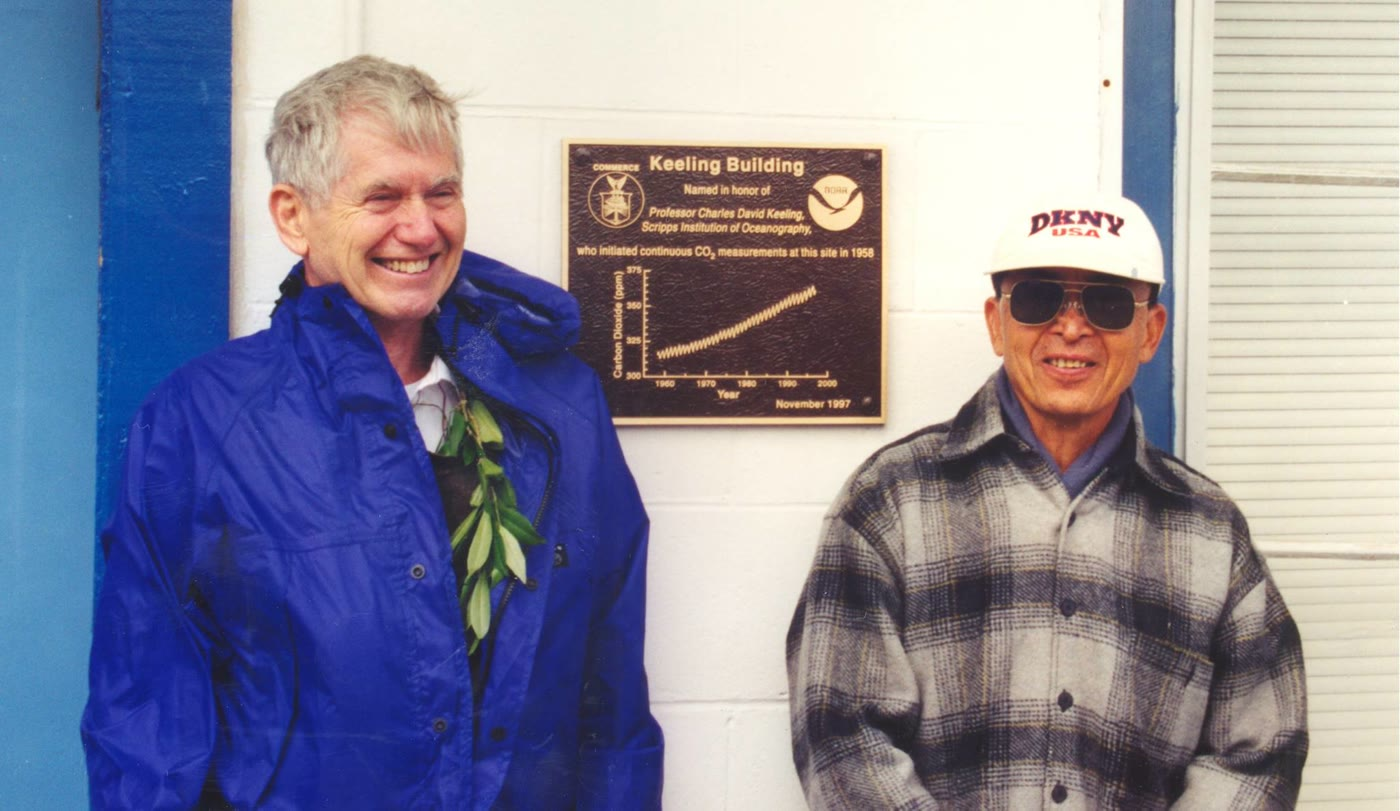
\includegraphics[width=0.62\linewidth]{images/book2/g12-noaa-keeling-chin-1997.jpg}

{\small Charles David Keeling (links) en John Chin in het Mauna Loa
Observatory in 1997, naast de plaquette die een gebouw naar Keeling vernoemt.
Foto: John Miller, NOAA (publiek domein).}
\end{center}
\end{history}

\section{Oefeningen}

\begin{exercise}[$\star$]\label{exo:g12:climate-change:1}
Wat is de \omterm{def:g12:climate-change:forcing}{stralingsforcering} van een verandering in het klimaatsysteem? In welke
eenheid wordt ze gemeten, en wat betekent haar teken?
\end{exercise}

\begin{exercise}[$\star$]\label{exo:g12:climate-change:2}
In welke maand van het jaar is de koolstofdioxideconcentratie op Mauna Loa
het hoogst, en in welke het laagst? Verklaar de jaarlijkse schommeling.
\end{exercise}

\begin{exercise}[$\star$]\label{exo:g12:climate-change:3}
Welke kans betekent \emph{zeer
waarschijnlijk} in de woordenschat van de evaluaties? En \emph{waarschijnlijk}? Wat betekent een bereik geschreven als
$[0.95 \text{ tot } 1.20]$?
\end{exercise}

\begin{exercise}[$\star$]\label{exo:g12:climate-change:4}
Welk deel van de extra energie die het klimaatsysteem de laatste decennia heeft gewonnen,
ging naar de oceaan? Waarom verklaart dit dat de zeespiegel stijgt,
zelfs zonder smeltend ijs?
\end{exercise}

\begin{exercise}[$\star$]\label{exo:g12:climate-change:5}
Geef twee positieve \omterm{def:g12:climate-change:feedback}{klimaatterugkoppelingen} en de negatieve reactie die
de opwarming begrenst. Leg elk uit in één zin.
\end{exercise}

\begin{exercise}[$\star\star$]\label{exo:g12:climate-change:6}
De jaargemiddelde concentratie koolstofdioxide op Mauna Loa was
\qty{315.98}{ppm} in 1959 en \qty{427.35}{ppm} in 2025. Met hoeveel ppm,
en met hoeveel procent, nam ze toe? Wat was de gemiddelde groei per
jaar over de hele periode?
\end{exercise}

\begin{exercise}[$\star\star$]\label{exo:g12:climate-change:7}
Gebruik de logaritmische wet van het hoofdstuk, met $F_{2\times} =
\qty{3.93}{W/m^2}$ en $C_0 = \qty{278}{ppm}$, om de \omterm{def:g12:climate-change:forcing}{forcering} van
koolstofdioxide bij \qty{427.35}{ppm}, het jaargemiddelde van 2025, te berekenen.
\end{exercise}

\begin{exercise}[$\star\star$]\label{exo:g12:climate-change:8}
Hoeveel zou de zeespiegel bij \qty{3.7}{mm} per jaar, de snelheid van 2006--2018,
in 30 jaar stijgen? Hoeveel keer sneller is deze snelheid dan die van
1901--1971, \qty{1.3}{mm} per jaar?
\end{exercise}

\begin{exercise}[$\star\star$]\label{exo:g12:climate-change:9}
Bereken met $\Delta T = F/\lambda$ en $\lambda = \qty{1.16}{W.m^{-2}.\degreeCelsius^{-1}}$
de evenwichtsopwarming die de totale menselijke \omterm{def:g12:climate-change:forcing}{forcering} van 2019,
\qty{2.72}{W/m^2}, zou veroorzaken. De waargenomen door de mens veroorzaakte opwarming is maar
ongeveer \qty{1.07}{\degreeCelsius}. Geef de belangrijkste reden voor het verschil.
\end{exercise}

\begin{exercise}[$\star\star$]\label{exo:g12:climate-change:10}
De Zon en vulkanen veranderden de mondiale temperatuur tussen 1850--1900 en
2010--2019 met $-0.1$ tot $+\qty{0.1}{\degreeCelsius}$, terwijl de waargenomen
opwarming ongeveer \qty{1.06}{\degreeCelsius} was. Wat kun je besluiten? Welke
andere natuurlijke oorzaak moet ook worden uitgesloten, en wat zegt de evaluatie
erover?
\end{exercise}

\begin{exercise}[$\star\star$]\label{exo:g12:climate-change:11}
Onder welke \omterm{def:g12:climate-change:scenario}{scenario's} blijft de opwarming van 2081--2100 volgens de tabel van \omterm{def:g12:climate-change:scenario}{projecties}
zeer waarschijnlijk onder \qty{2}{\degreeCelsius}? Onder welke
overschrijdt ze \qty{2}{\degreeCelsius} zeer waarschijnlijk?
\end{exercise}

\begin{exercise}[$\star\star\star$]\label{exo:g12:climate-change:12}
Aerosolen veroorzaakten een \omterm{def:g12:climate-change:forcing}{forcering} van ongeveer $-0.22$ en $\qty{-0.84}{W/m^2}$
(via zonlicht en via wolken). Als alle aerosolen uit de
lucht werden verwijderd terwijl al het andere bleef zoals in 2019, wat zou de totale menselijke
\omterm{def:g12:climate-change:forcing}{forcering} dan worden? Met hoeveel zou de evenwichtsopwarming toenemen, met
$\lambda = \qty{1.16}{W.m^{-2}.\degreeCelsius^{-1}}$?
\end{exercise}

\begin{exercise}[$\star\star\star$]\label{exo:g12:climate-change:13}
Toon met de logaritmische wet aan dat de stap van \qty{278}{ppm} naar
\qty{556}{ppm} en de stap van \qty{556}{ppm} naar \qty{1112}{ppm} dezelfde
\omterm{def:g12:climate-change:forcing}{forcering} toevoegen. Wat is de totale \omterm{def:g12:climate-change:forcing}{forcering} bij \qty{1112}{ppm}?
\end{exercise}

\begin{exercise}[$\star\star\star$]\label{exo:g12:climate-change:14}
Leid de logaritmische wet af naar $C$. Hoeveel \omterm{def:g12:climate-change:forcing}{forcering} voegt
één extra ppm koolstofdioxide toe bij \qty{280}{ppm}, en hoeveel bij
\qty{420}{ppm}? Geef commentaar.
\end{exercise}

\begin{exercise}[$\star\star\star$]\label{exo:g12:climate-change:15}
Zonder enige \omterm{def:g12:climate-change:feedback}{terugkoppeling} behalve de extra straling naar de ruimte is
$\lambda_0 = \qty{3.22}{W.m^{-2}.\degreeCelsius^{-1}}$. Bereken de opwarming
voor een verdubbeling van koolstofdioxide ($F_{2\times} = \qty{3.93}{W/m^2}$) met
$\lambda_0$, en dan met $\lambda = \qty{1.16}{W.m^{-2}.\degreeCelsius^{-1}}$. Met
welke factor versterken de \omterm{def:g12:climate-change:feedback}{terugkoppelingen} de opwarming?
\end{exercise}

\section{Probleem: De Keelingcurve in cijfers}

\begin{problem}[{Weekendprobleem --- van het jaarlijkse ademen van de
begroeiing tot het jaar waarin een verdubbeling zou worden bereikt}]
\label{pb:g12:climate-change:1}
% ledger: data:co2-mlo (annual means 1960 316.91, 1970 325.68, 2015 401.01,
% 2025 427.35; seasonal departures May +3.37, September -3.51, means of
% 2015-2024; all from figdata/grade-12/climate_records.py), noaa:mlo-site,
% ipcc:erf-2xco2, ipcc:ecs, ipcc:feedbacks, ipcc:co2-2myr
Een leerling downloadt de reeks van Mauna Loa en werkt ze door met een
rekenblad. Over 2015--2024 ligt de maandelijkse concentratie gemiddeld
\qty{3.37}{ppm} boven de afgevlakte trend in mei en \qty{3.51}{ppm} eronder
in september. De jaargemiddelden zijn \qty{316.91}{ppm} in 1960,
\qty{325.68}{ppm} in 1970, \qty{401.01}{ppm} in 2015 en \qty{427.35}{ppm}
in 2025. De concentratie van 1750 was \qty{278}{ppm}. Gebruik de logaritmische
wet met $F_{2\times} = \qty{3.93}{W/m^2}$.

\medskip
\noindent\textbf{Deel I --- Het ademen van de begroeiing.}
\begin{enumerate}
  \item Wat is de amplitude van top tot dal van de jaarlijkse cyclus?
  \item Verklaar waarom de concentratie het hoogst is in mei en het laagst in
        september.
  \item De cyclus is veel zwakker in de lucht van het zuidelijk halfrond.
        Opper een verklaring.
  \item Waarom werd het observatorium op \qty{3397}{m} hoogte gebouwd, op een vulkaan
        midden in de Grote Oceaan?
\end{enumerate}

\medskip
\noindent\textbf{Deel II --- De trend.}
\begin{enumerate}[resume]
  \item Bereken de gemiddelde groei, in ppm per jaar, over 1960--1970.
  \item Bereken ze over 2015--2025.
  \item Met welke factor is de groeisnelheid toegenomen?
  \item Met hoeveel procent steeg de concentratie tussen 1750 en
        2025?
  \item De \omterm{def:g12:past-climates:ice-core}{ijskernen} tonen over de laatste 800\,000 jaar nooit meer dan ongeveer \qty{300}{ppm}.
        Met hoeveel ppm overschrijdt de waarde van 2025
        dit?
\end{enumerate}

\medskip
\noindent\textbf{Deel III --- De forcering.}
\begin{enumerate}[resume]
  \item Bereken de \omterm{def:g12:climate-change:forcing}{forcering} van koolstofdioxide in 2025.
  \item Bereken ze in 1960, en de toename van de \omterm{def:g12:climate-change:forcing}{forcering} tussen 1960
        en 2025.
  \item Welke concentratie zou \qty{1}{W/m^2} toevoegen aan de \omterm{def:g12:climate-change:forcing}{forcering} van 2025?
  \item Hoeveel jaar zou dat duren bij de groeisnelheid van 2015--2025?
\end{enumerate}

\medskip
\noindent\textbf{Deel IV --- De verdubbeling.}
\begin{enumerate}[resume]
  \item Wat is de concentratie bij een verdubbeling van de waarde van 1750? Welke
        \omterm{def:g12:climate-change:forcing}{forcering} levert ze?
  \item Welke evenwichtsopwarming zou ze veroorzaken bij de beste schatting van de \omterm{def:g12:climate-change:ecs}{evenwichtsklimaatgevoeligheid}?
        Geef het waarschijnlijke bereik.
  \item Welke terugkoppelingsparameter $\lambda$ volgt uit een gevoeligheid van
        \qty{3}{\degreeCelsius}? Vergelijk hem met de waarde
        \qty{1.16}{W.m^{-2}.\degreeCelsius^{-1}} die je krijgt door de
        \omterm{def:g12:climate-change:feedback}{terugkoppelingen} op te tellen.
  \item Waarom zou het oppervlak deze opwarming niet bereiken op de dag dat de
        verdubbeling wordt bereikt?
  \item Waarom is een berekening die gewoon de huidige groeisnelheid doortrekt een
        \omterm{def:g12:climate-change:scenario}{scenario}, en geen \omterm{def:g12:climate-change:scenario}{projectie} van het soort dat de evaluaties maken?
  \item In welk jaar zou de verdubbeling van de concentratie van 1750 worden bereikt
        als de groeisnelheid van 2015--2025 dezelfde bleef?
\end{enumerate}
\end{problem}
